\documentclass[aspectratio=169,12pt]{beamer}
\usetheme{Madrid}
\usecolortheme{dolphin}
\usefonttheme{professionalfonts}
\setbeamertemplate{navigation symbols}{}
\setbeamertemplate{footline}{}

\usepackage[T1]{fontenc}
\usepackage[utf8]{inputenc}
\usepackage{graphicx}
\usepackage{amsmath,amssymb}
\usepackage{hyperref}
\usepackage{siunitx}
\usepackage{physics}
\usepackage{braket}

\graphicspath{{../../figures/}}

\title[Module B6]{Module B6: Algorithme de Grover}
\author{JAMOTTE Maxime, SCHOONEN Cédric}
\institute{Digital Learning Hub}
\date{}

\begin{document}

\begin{frame}
  \titlepage
\end{frame}

\begin{frame}{Algorithme de Grover (voir JN)}
  \begin{itemize}
    \setlength{\itemsep}{0.8em}
    \item Problème de recherche: identifier une entrée dans une base de données non-structurée.\\~\\
    \item On encode les solutions possibles sur $n$ qubits ($N = 2^n$ valeurs possibles).\\~\\
    \item Concept d'\textbf{oracle}: une opération qui identifie la solution recherchée.\\~\\
    \item L'\textbf{itération de Grover} amplifie la probabilité de mesurer la bonne solution.\\~\\
    \item Complexité: $O(\sqrt{N})$ évaluations au lieu de $O(N)$ classiquement.
  \end{itemize}
\end{frame}

\begin{frame}{Aspect géométrique}
  \begin{itemize}[<+->]
    \setlength{\itemsep}{0.8em}
    \item L'état initial est une superposition uniforme de tous les états.\\~\\
    \item L'oracle inverse le signe de l'amplitude de la solution.\\~\\
    \item L'opérateur de diffusion amplifie l'amplitude de la solution.\\~\\
    \item Chaque itération fait tourner le vecteur d'un angle $2\theta$ vers la solution.
  \end{itemize}
\end{frame}

\begin{frame}{Circuit de Grover}
  \begin{center}
    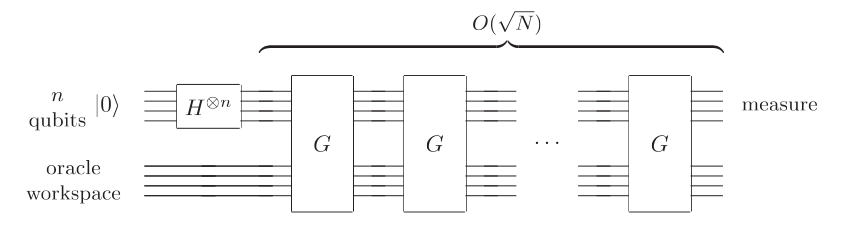
\includegraphics[width=0.9\textwidth]{grover_full.png}
  \end{center}
\end{frame}

\begin{frame}{Itération de Grover}
  \begin{center}
    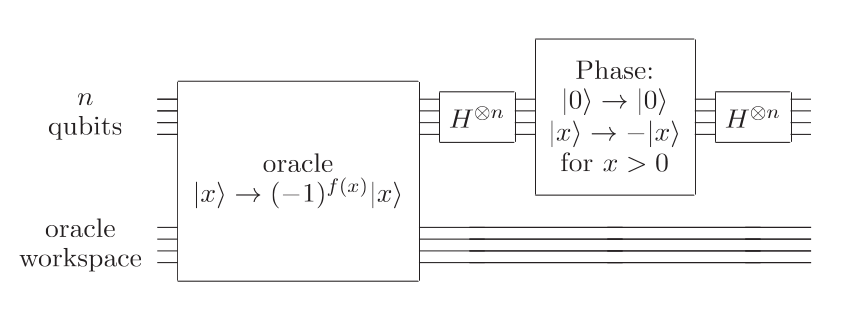
\includegraphics[width=0.9\textwidth]{grover_iter.png}
  \end{center}
\end{frame}

\begin{frame}{Implémentation avec Qiskit (voir JN)}
  \begin{itemize}
    \setlength{\itemsep}{0.8em}
    \item Construction de l'oracle identifiant un état particulier.\\~\\
    \item Construction de l'opérateur de diffusion avec portes de Hadamard.\\~\\
    \item Application des itérations de Grover.\\~\\
    \item Mesure et vérification des résultats.\\~\\
    \item Voir le Jupyter Notebook pour l'implémentation complète.
  \end{itemize}
\end{frame}

\begin{frame}{Fin du module B6}
  \centering
  \vfill
  Module optionnel recommandé.
  \vfill
\end{frame}

\end{document}
